\documentclass[aspectratio=169]{beamer}
\usetheme{Madrid}
\usecolortheme{default}

\usepackage[utf8]{inputenc}
\usepackage[english]{babel}
\usepackage{graphicx}
\usepackage{booktabs}
\usepackage{amsmath}
\usepackage[table]{xcolor}
\usepackage{tikz}
\usepackage{pgfplots}
\pgfplotsset{compat=1.18}

\definecolor{cvutblue}{RGB}{0,101,189}
\definecolor{lightgreen}{RGB}{200,255,200}
\definecolor{lightyellow}{RGB}{255,255,200}
\definecolor{darkgreen}{RGB}{0,128,0}
\definecolor{lightblue}{RGB}{200,220,255}
\definecolor{lightorange}{RGB}{255,220,180}
\definecolor{lightpurple}{RGB}{220,200,255}
\definecolor{verylightyellow}{RGB}{255,255,220}
\setbeamercolor{structure}{fg=cvutblue}

\title{Warehouse Layout Optimization}
\subtitle{EA with Surrogate Models, Feature Selection and Ensemble Methods}
\author{David Zeman, Petr Šmíd, Dita Chabičovská}
\institute{MFF UK}
\date{2026}

\begin{document}

\begin{frame}
\titlepage
\end{frame}

%===============================================================================
\section{Problem}
%===============================================================================

\begin{frame}{Problem}
\begin{columns}
\begin{column}{0.55\textwidth}
\begin{itemize}
    \item Warehouse $9 \times 9$, 49 product positions, 4 agents
    \item Order distribution: Zipf 1.2
    \item Goal: find layout maximizing throughput
    \item Search space: $49! \approx 6 \times 10^{62}$ permutations
    \item One simulation: 2--3s
\end{itemize}

\vspace{0.5cm}
\textbf{Surrogate model:}
\begin{itemize}
    \item 40 features from layout $\rightarrow$ fitness prediction
    \item Hybrid EA: surrogate + occasional real evaluations
\end{itemize}
\end{column}
\begin{column}{0.45\textwidth}
\centering
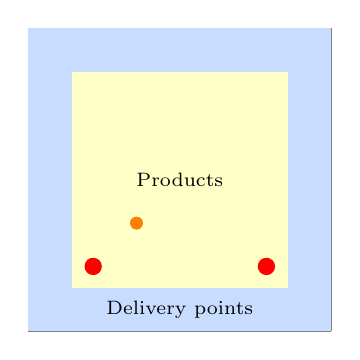
\begin{tikzpicture}[scale=0.55]
    \draw[step=1, gray, thin] (0,0) grid (7,7);
    \fill[lightblue] (0,0) rectangle (7,1);
    \fill[lightblue] (0,6) rectangle (7,7);
    \fill[lightblue] (0,1) rectangle (1,6);
    \fill[lightblue] (6,1) rectangle (7,6);
    \fill[lightyellow] (1,1) rectangle (6,6);
    \node at (3.5, 0.5) {\scriptsize Delivery points};
    \node at (3.5, 3.5) {\scriptsize Products};
    \fill[red] (1.5, 1.5) circle (0.2);
    \fill[red] (5.5, 1.5) circle (0.2);
    \fill[orange] (2.5, 2.5) circle (0.15);
\end{tikzpicture}

\vspace{0.2cm}
\scriptsize Red = popular products
\end{column}
\end{columns}
\end{frame}

%===============================================================================
\section{MAPD}
%===============================================================================

\begin{frame}{MAPD -- Multi-Agent Pickup and Delivery}
\begin{columns}
\begin{column}{0.55\textwidth}
\textbf{Problem:}
\begin{itemize}
    \item $k$ agents, infinite stream of tasks
    \item Task = pickup product + deliver to output
    \item Agents must not collide
    \item Goal: maximize throughput
\end{itemize}

\vspace{0.4cm}
\textbf{Our approach:}
\begin{itemize}
    \item \textbf{Token Passing} -- decentralized task assignment
    \item \textbf{A* planner} -- pathfinding for each agent
    \item Reservation table -- collision prevention
\end{itemize}

\vspace{0.4cm}
\textbf{Fitness function:}
\begin{itemize}
    \item $\text{fitness} = \frac{\text{completed tasks}}{\text{simulation time}}$
    \item Throughput = deliveries per time unit
    \item Higher = better (layout enables more deliveries)
\end{itemize}
\end{column}
\begin{column}{0.45\textwidth}
\centering
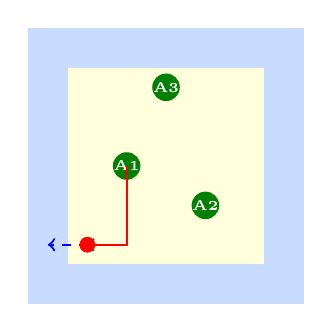
\begin{tikzpicture}[scale=0.5]
    % Grid
    \draw[step=1, gray, thin] (0,0) grid (7,7);
    % Delivery points
    \fill[lightblue] (0,0) rectangle (7,1);
    \fill[lightblue] (0,6) rectangle (7,7);
    \fill[lightblue] (0,1) rectangle (1,6);
    \fill[lightblue] (6,1) rectangle (7,6);
    % Inner
    \fill[verylightyellow] (1,1) rectangle (6,6);

    % Agents
    \fill[darkgreen] (2.5, 3.5) circle (0.35);
    \node[white, font=\tiny\bfseries] at (2.5, 3.5) {A1};
    \fill[darkgreen] (4.5, 2.5) circle (0.35);
    \node[white, font=\tiny\bfseries] at (4.5, 2.5) {A2};
    \fill[darkgreen] (3.5, 5.5) circle (0.35);
    \node[white, font=\tiny\bfseries] at (3.5, 5.5) {A3};

    % Path example
    \draw[->, red, thick] (2.5, 3.5) -- (2.5, 1.5) -- (1.5, 1.5);
    \draw[->, blue, thick, dashed] (1.5, 1.5) -- (0.5, 1.5);

    % Target
    \fill[red] (1.5, 1.5) circle (0.2);
\end{tikzpicture}

\vspace{0.3cm}
\scriptsize
Green = agents\\
Red = target (pickup)\\
Blue = path to delivery
\end{column}
\end{columns}
\end{frame}

%===============================================================================
\section{Feature Selection}
%===============================================================================

\begin{frame}{Extracted Features (40)}
\begin{columns}
\begin{column}{0.5\textwidth}
\textbf{Distance-based (10):}
\begin{itemize}
    \item Weighted mean/std distance to edge
    \item Min/max/avg distance of top items
    \item Weighted quadratic distance
\end{itemize}

\vspace{0.3cm}
\textbf{Position-based (8):}
\begin{itemize}
    \item Number of popular items on edge
    \item Proportion in corners
    \item Quadrant distribution (NW, NE, SW, SE)
\end{itemize}
\end{column}
\begin{column}{0.5\textwidth}
\textbf{Distribution-based (6):}
\begin{itemize}
    \item Entropy, Gini coefficient
    \item Probability mass on edge/center
    \item Median, 90th percentile, skewness
\end{itemize}

\vspace{0.3cm}
\textbf{Congestion/clustering (10):}
\begin{itemize}
    \item Congestion score, hotspot
    \item Local density, dispersion
    \item Bottleneck, path overlap
    \item Spread X/Y, quadrant balance
\end{itemize}

\vspace{0.3cm}
\textbf{Delivery-based (6):}
\begin{itemize}
    \item Distance to delivery points
    \item Number of accessible delivery points
\end{itemize}
\end{column}
\end{columns}
\end{frame}

\begin{frame}{Feature Selection}
\begin{columns}
\begin{column}{0.5\textwidth}
\centering
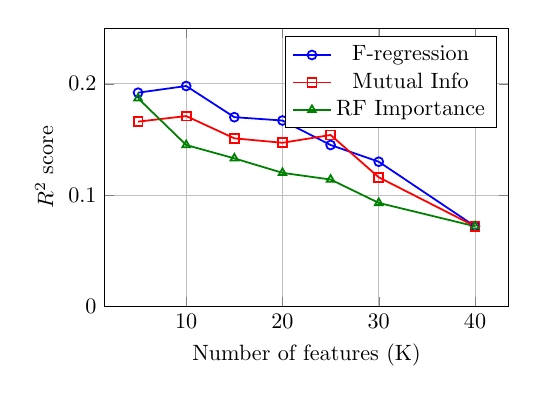
\begin{tikzpicture}[scale=0.8]
\begin{axis}[
    xlabel={Number of features (K)},
    ylabel={$R^2$ score},
    legend pos=north east,
    grid=major,
    ymin=0, ymax=0.25,
    width=8cm, height=6cm
]
\addplot[blue, mark=o, thick] coordinates {
    (5, 0.192) (10, 0.198) (15, 0.170) (20, 0.167) (25, 0.145) (30, 0.130) (40, 0.072)
};
\addlegendentry{F-regression}

\addplot[red, mark=square, thick] coordinates {
    (5, 0.166) (10, 0.171) (15, 0.151) (20, 0.147) (25, 0.154) (30, 0.116) (40, 0.072)
};
\addlegendentry{Mutual Info}

\addplot[darkgreen, mark=triangle, thick] coordinates {
    (5, 0.187) (10, 0.145) (15, 0.133) (20, 0.120) (25, 0.114) (30, 0.093) (40, 0.072)
};
\addlegendentry{RF Importance}
\end{axis}
\end{tikzpicture}
\end{column}
\begin{column}{0.5\textwidth}
\textbf{Top 5 features (RF importance):}
\begin{enumerate}
    \item \texttt{edge\_prob\_mass} (0.142)
    \item \texttt{dist\_gini} (0.059)
    \item \texttt{quad\_SE} (0.050)
    \item \texttt{spread\_x} (0.050)
    \item \texttt{quad\_NW} (0.044)
\end{enumerate}

\vspace{0.5cm}
\begin{alertblock}{Result}
\begin{itemize}
    \item Optimum: \textbf{K = 10} features
    \item $R^2$: 0.072 $\rightarrow$ \textbf{0.198} (+175\%)
\end{itemize}
\end{alertblock}
\end{column}
\end{columns}
\end{frame}

%===============================================================================
\section{Ensemble Models}
%===============================================================================

\begin{frame}{Ensemble Surrogate}
\begin{columns}
\begin{column}{0.5\textwidth}
\textbf{Voting Ensemble:}
\begin{itemize}
    \item Ridge + RF + GBM
    \item Output = average of predictions
\end{itemize}

\vspace{0.3cm}
\textbf{Stacking Ensemble:}
\begin{itemize}
    \item Ridge + RF + GBM
    \item Meta-learner combines predictions
\end{itemize}

\vspace{0.5cm}
\centering
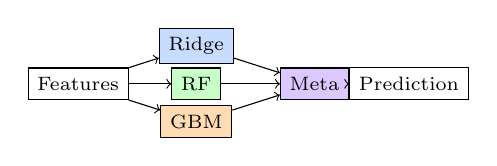
\begin{tikzpicture}[scale=0.6, every node/.style={font=\scriptsize}]
    \node[draw, rectangle] (input) at (0,0) {Features};
    \node[draw, rectangle, fill=lightblue] (ridge) at (2.5,0.8) {Ridge};
    \node[draw, rectangle, fill=lightgreen] (rf) at (2.5,0) {RF};
    \node[draw, rectangle, fill=lightorange] (gbm) at (2.5,-0.8) {GBM};
    \node[draw, rectangle, fill=lightpurple] (meta) at (5,0) {Meta};
    \node[draw, rectangle] (output) at (7,0) {Prediction};
    \draw[->] (input) -- (ridge);
    \draw[->] (input) -- (rf);
    \draw[->] (input) -- (gbm);
    \draw[->] (ridge) -- (meta);
    \draw[->] (rf) -- (meta);
    \draw[->] (gbm) -- (meta);
    \draw[->] (meta) -- (output);
\end{tikzpicture}
\end{column}
\begin{column}{0.5\textwidth}
\centering
\textbf{$R^2$ Comparison (CV):}

\vspace{0.3cm}
\begin{tabular}{lc}
\toprule
\textbf{Model} & \textbf{$R^2$} \\
\midrule
\rowcolor{lightgreen} Voting (10 feat.) & $0.166$ \\
GP (40 feat.) & $0.152$ \\
Ridge (10 feat.) & $0.145$ \\
RF (40 feat.) & $0.145$ \\
Stacking (10 feat.) & $0.123$ \\
Ridge (40 feat.) & $0.072$ \\
\bottomrule
\end{tabular}
\end{column}
\end{columns}
\end{frame}

%===============================================================================
\section{Results}
%===============================================================================

\begin{frame}{Main Results}
\begin{columns}
\begin{column}{0.55\textwidth}
\centering
\begin{tabular}{lcc}
\toprule
\textbf{Method} & \textbf{Fitness} & \textbf{Time} \\
\midrule
Random (best) & 0.48 & -- \\
Greedy & 0.44 & -- \\
\midrule
EA without surrogate & 0.55 & 43 min \\
EA + Voting & 0.56 & 7.5 min \\
\rowcolor{lightgreen} \textbf{EA + Stacking} & \textbf{0.58} & \textbf{10.5 min} \\
\bottomrule
\end{tabular}

\vspace{0.5cm}
\small
Real evaluations: 1020 $\rightarrow$ \textbf{168} (--83.5\%)
\end{column}
\begin{column}{0.45\textwidth}
\begin{block}{Best: EA + Stacking}
\begin{itemize}
    \item Fitness \textbf{0.58} (+5.5\% vs EA)
    \item \textbf{4$\times$ faster} than EA without surrogate
    \item +21\% over Greedy baseline
\end{itemize}
\end{block}

\vspace{0.3cm}
\begin{alertblock}{Key Conclusion}
Ensemble surrogate + feature selection = better results in less time
\end{alertblock}
\end{column}
\end{columns}
\end{frame}

\begin{frame}{Convergence}
\begin{columns}
\begin{column}{0.5\textwidth}
\centering
\textbf{Fitness vs. Generation}
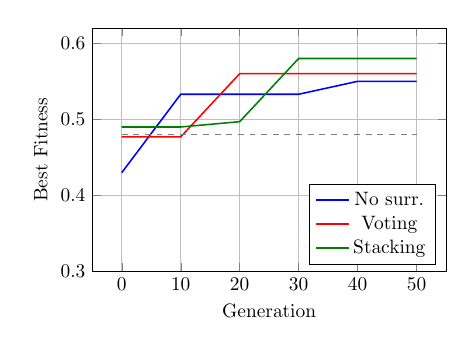
\begin{tikzpicture}[scale=0.7]
\begin{axis}[
    xlabel={Generation},
    ylabel={Best Fitness},
    legend pos=south east,
    grid=major,
    width=8cm, height=6cm,
    ymin=0.3, ymax=0.62
]
\addplot[blue, thick] coordinates {
    (0, 0.43) (10, 0.533) (20, 0.533) (30, 0.533) (40, 0.55) (50, 0.55)
};
\addlegendentry{No surr.}

\addplot[red, thick] coordinates {
    (0, 0.477) (10, 0.477) (20, 0.56) (30, 0.56) (40, 0.56) (50, 0.56)
};
\addlegendentry{Voting}

\addplot[darkgreen, thick] coordinates {
    (0, 0.49) (10, 0.49) (20, 0.497) (30, 0.58) (40, 0.58) (50, 0.58)
};
\addlegendentry{Stacking}

\addplot[gray, dashed] coordinates {(0, 0.48) (50, 0.48)};
\end{axis}
\end{tikzpicture}
\end{column}
\begin{column}{0.5\textwidth}
\centering
\textbf{Fitness vs. Time}
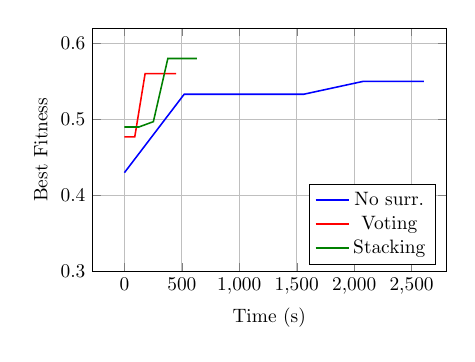
\begin{tikzpicture}[scale=0.7]
\begin{axis}[
    xlabel={Time (s)},
    ylabel={Best Fitness},
    legend pos=south east,
    grid=major,
    width=8cm, height=6cm,
    ymin=0.3, ymax=0.62,
    xmax=2800
]
\addplot[blue, thick] coordinates {
    (0, 0.43) (520, 0.533) (1040, 0.533) (1560, 0.533) (2080, 0.55) (2608, 0.55)
};
\addlegendentry{No surr.}

\addplot[red, thick] coordinates {
    (0, 0.477) (90, 0.477) (180, 0.56) (270, 0.56) (360, 0.56) (451, 0.56)
};
\addlegendentry{Voting}

\addplot[darkgreen, thick] coordinates {
    (0, 0.49) (126, 0.49) (252, 0.497) (378, 0.58) (504, 0.58) (630, 0.58)
};
\addlegendentry{Stacking}
\end{axis}
\end{tikzpicture}
\end{column}
\end{columns}
\end{frame}

%===============================================================================
\section{Conclusion}
%===============================================================================

\begin{frame}{Conclusion}

\begin{center}
\Large\textbf{Surrogate model significantly accelerates EA optimization}
\end{center}

\vspace{0.5cm}

\begin{columns}[T]
\begin{column}{0.48\textwidth}
\begin{block}{What we did}
\begin{itemize}
    \item Feature selection: 40 → 10 features
    \item Ensemble surrogate models
    \item Integration into EA optimization
\end{itemize}
\end{block}
\end{column}

\begin{column}{0.48\textwidth}
\begin{block}{What we achieved}
\begin{itemize}
    \item \textbf{4--6$\times$ faster} optimization
    \item \textbf{83\% fewer} simulations
    \item \textbf{Better fitness} than baseline
\end{itemize}
\end{block}
\end{column}
\end{columns}

\vspace{0.5cm}

\begin{alertblock}{Recommendation}
\textbf{Stacking ensemble} -- best solution quality (fitness 0.58)\\
\textbf{Voting ensemble} -- fastest variant (5.8$\times$ speedup)
\end{alertblock}

\end{frame}

\end{document}
